\RequirePackage{fix-cm}
%
\RequirePackage{amsmath}



%\documentclass{svjour3}                     % onecolumn (standard format)
%\documentclass[smallcondensed]{svjour3}     % onecolumn (ditto)
%\documentclass[smallextended]{svjour3}       % onecolumn (second format)
% \documentclass[twocolumn]{svjour3}          % twocolumn
%\documentclass[letterpaper, 12pt, twocolumn]{article}
\documentclass{article}
\usepackage[cm]{fullpage}
%\usepackage[margin=1in]{geometry}
\usepackage{amssymb}
\usepackage{graphicx}
\usepackage[utf8]{inputenc}
\usepackage{indentfirst}
%\usepackage{physics}
\newcommand{\me}{\mathrm{e}}
\usepackage{amsmath}

%\usepackage[monochrome]{color}

%\usepackage[round]{natbib}
%\usepackage{apacite}
\usepackage{url}


\PassOptionsToPackage{monochrome}{xcolor}

% For the flow charts
\usepackage{tikz}
\usetikzlibrary{
	external,
}
\tikzexternalize

\usetikzlibrary{shapes.geometric, arrows, calc, positioning}
\tikzstyle{startstop} = [rectangle, thick, rounded corners=2.5mm, minimum width=2cm, minimum height=5mm,text centered, draw=black]
\tikzstyle{io} = [trapezium, thick, trapezium left angle=70, trapezium right angle=110, text width=3.75cm, minimum height=0.5cm, text centered, draw=black]
\tikzstyle{process} = [rectangle, thick, minimum width=2.5cm, text width=4cm, minimum height=0.5cm, text centered, draw=black]
\tikzstyle{block} = [rectangle, thick, minimum width=0.5cm, minimum height=1cm, text centered, draw=black]
\tikzstyle{support} = [coordinate, join=by fuzzy]
\tikzstyle{decision} = [diamond, thick, minimum width=3cm, minimum height=1cm, text centered, draw=black]
\tikzstyle{dottedbox} = [rectangle, dotted, thick, minimum width=2.5cm, text width=2.8cm, minimum height=0.5cm, text centered, draw=black]
\tikzstyle{arrow} = [thick,->,>=stealth]
\tikzstyle{dottedarrow} = [thick, dotted,->,>=stealth]





\usepackage{pgfplots}
\usepgfplotslibrary{patchplots}
\pgfplotsset{compat=newest, samples=015} %Set this value to 65 for the final version
%\usepgfplotslibrary{dateplot} 


%\providecommand{\keywords}[1]{\textbf{\textit{Index terms---}} #1}

%\journalname{Journal of Science Education and Technology}

\begin{document}


\title{Algorithm to generate multi-factorial experiments to teach experimental design%\thanks{Grants or other notes
%about the article that should go on the front page should be
%placed here. General acknowledgments should be placed at the end of the article.}
}
%\subtitle{Do you have a subtitle?\\ If so, write it here}
%\titlerunning{Short form of title}        % if too long for running head
\author{A.C.~Delgado-Chavez  \and
        N.~Balagurusamy \and
        R.~Narayanasamy \and
        S.~K.~Gadi
}

\begin{figure}
	\centering
	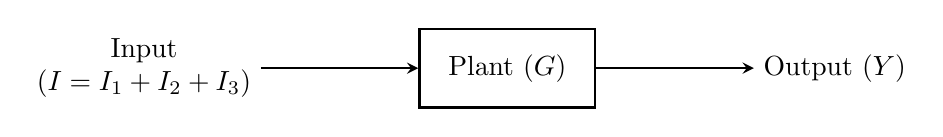
\begin{tikzpicture}[node distance = 10mm, auto]
		\node (Input) [align=center] {Input\\($I=I_1+I_2+I_3$)};
		\node (Plant) [block, text width = 2cm, right = 2cm of Input] {Plant ($G$)};
		\node (Output) [right = of Plant, right = 2cm] {Output ($Y$)};
		\draw [arrow] (Input) -- (Plant);
		\draw [arrow] (Plant) -- (Output);
	\end{tikzpicture}
	\caption{Open loop system}
	\label{Fig:OpenLoop}
\end{figure}

\begin{figure}
	\centering
	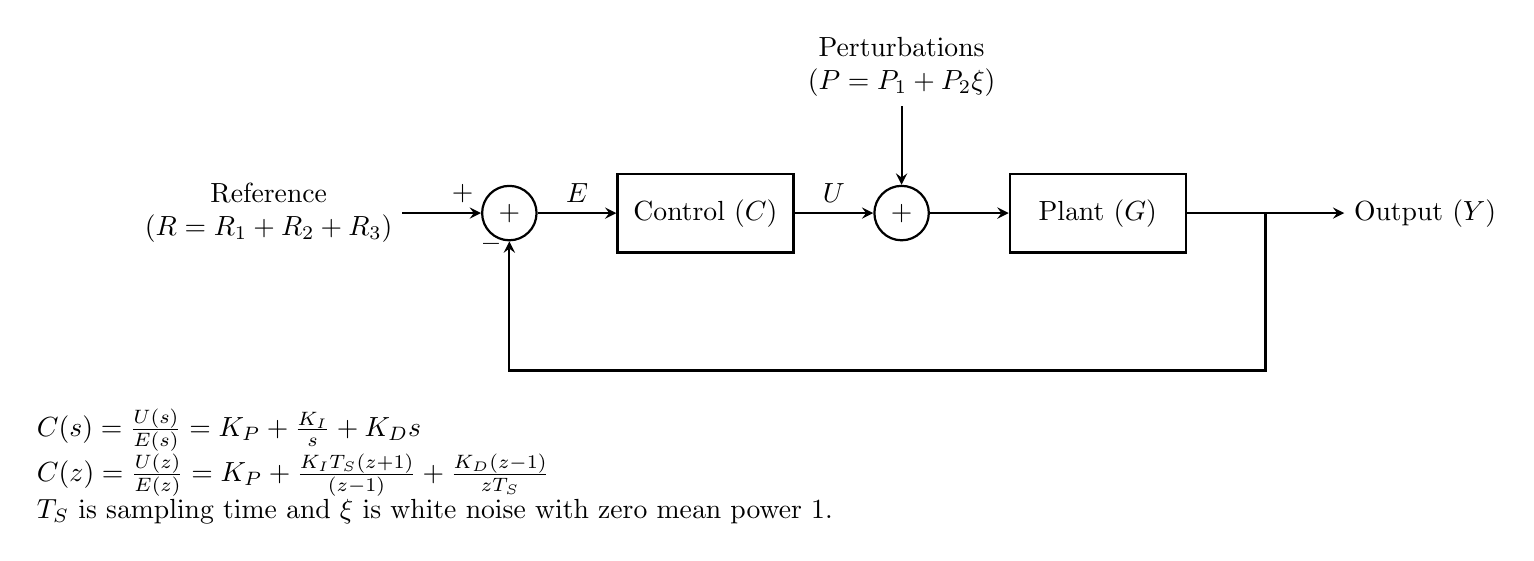
\begin{tikzpicture}[node distance = 10mm, auto]
	\node (Reference) [align=center] {Reference\\($R=R_1+R_2+R_3$)};
	\node (SummingPoint) [draw,circle, thick, right = of Reference]  {+};
	\node (Control) [block, text width = 2cm, right = of SummingPoint] {Control ($C$)};
	\node (SummingPoint1) [draw,circle, thick, right = of Control]  {+};
	\node (Plant) [block, text width = 2cm, right = of SummingPoint1] {Plant ($G$)};
	\node (PlantRight) [support, right = of Plant, right = 1cm] {};
	\node (Output) [right = of Plant, right = 2cm] {Output ($Y$)};
	\node (Perturbations) [align=center, above = of SummingPoint1] {Perturbations\\($P=P_1+P_2\xi$)};
	\draw [arrow] (Reference) -- node[anchor=south west]{+}(SummingPoint);
	\draw [arrow] (SummingPoint) -- node[anchor=south]{$E$}(Control);
	\draw [arrow] (Control) -- node[anchor=south]{$U$}(SummingPoint1);
	\draw [arrow] (SummingPoint1) -- (Plant);
	\draw [arrow] (Plant) -- (Output);
	\draw [arrow] (PlantRight) -- +(0, -2) -| (SummingPoint) node[below = 2mm, anchor=north east]{\bf\textendash};
	\draw [arrow] (Perturbations) -- (SummingPoint1);
	\node (Equation000) [text width = 12cm, below = 2cm of SummingPoint, align = left] {
		$C(s) = \frac{U(s)}{E(s)} = K_P + \frac{K_I}{s} + K_Ds$\\
		$C(z) = \frac{U(z)}{E(z)} = K_P + \frac{K_IT_S(z+1)}{(z-1)} + \frac{K_D(z-1)}{zT_S}$\\
		$T_S$ is sampling time and $\xi$ is white noise with zero mean power 1.
	};
	\end{tikzpicture}
	\caption{Closed loop system with a PID Controller}
	\label{Fig:PID}
\end{figure}

\begin{figure}
	\centering
	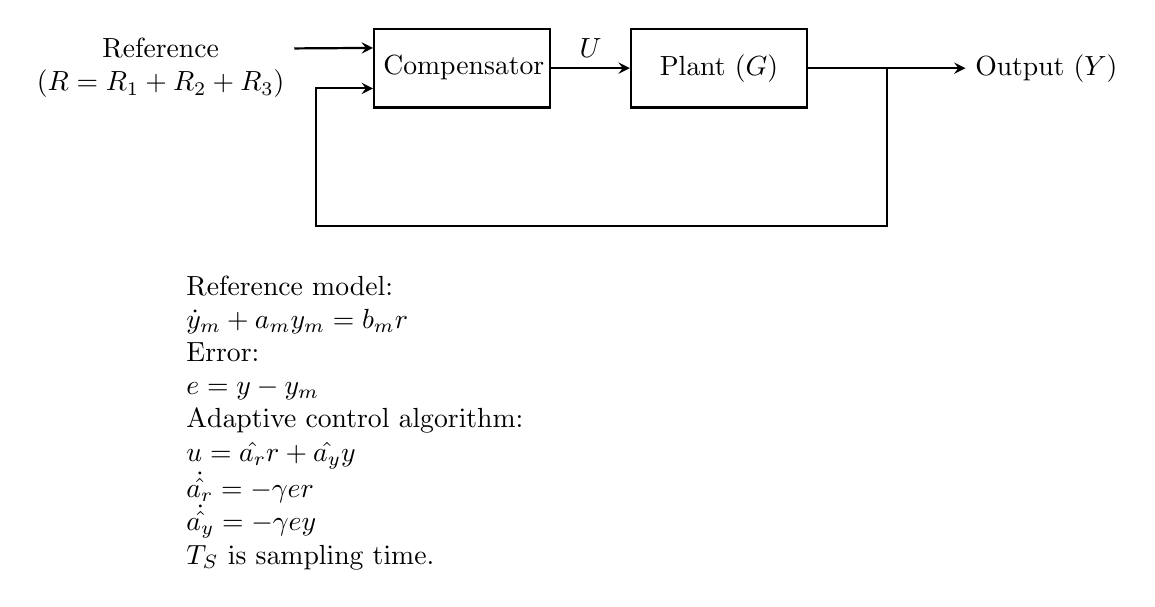
\begin{tikzpicture}[node distance = 10mm, auto]
	\node (Reference) [align=center] {Reference\\($R=R_1+R_2+R_3$)};
	\node (Control) [block, text width = 2cm, right = of Reference] {Compensator};
	\node (Plant) [block, text width = 2cm, right = of Control] {Plant ($G$)};
	\node (PlantRight) [support, right = of Plant, right = 1cm] {};
	\node (Output) [right = of Plant, right = 2cm] {Output ($Y$)};
	\path (Reference.east) -- (Reference.north east) coordinate[pos=0.5] (Reference1);
	\path (Control.west) -- (Control.north west) coordinate[pos=0.5] (Control1);
	\path (Control.west) -- (Control.north west) coordinate[pos=-0.5] (Control2);
	\draw [arrow] (Reference1) -- (Control1);
	\draw [arrow] (Control) -- node[anchor=south]{$U$}(Plant);
	\draw [arrow] (Plant) -- (Output);
	\draw [arrow] (PlantRight) -- +(0, -2) -| +(-7.25,-2) |- (Control2);
	\node (Equation000) [text width = 7cm, below = 2cm of Control, align = left] {
		Reference model:\\
		$\dot y_m + a_m y_m = b_mr$\\
		Error:\\
		$e = y-y_m$\\
		Adaptive control algorithm:\\
		$u = \hat{a_r} r + \hat{a_y}y$\\
		$\dot{\hat{a_r}} = - \gamma e r$\\
		$\dot{\hat{a_y}} = - \gamma e y$\\
		$T_S$ is sampling time.
	};
	\end{tikzpicture}
	\caption{Closed loop system with an Adaptive controller}
	\label{Fig:AdaptiveControl}
\end{figure}


\begin{figure}
	\centering
	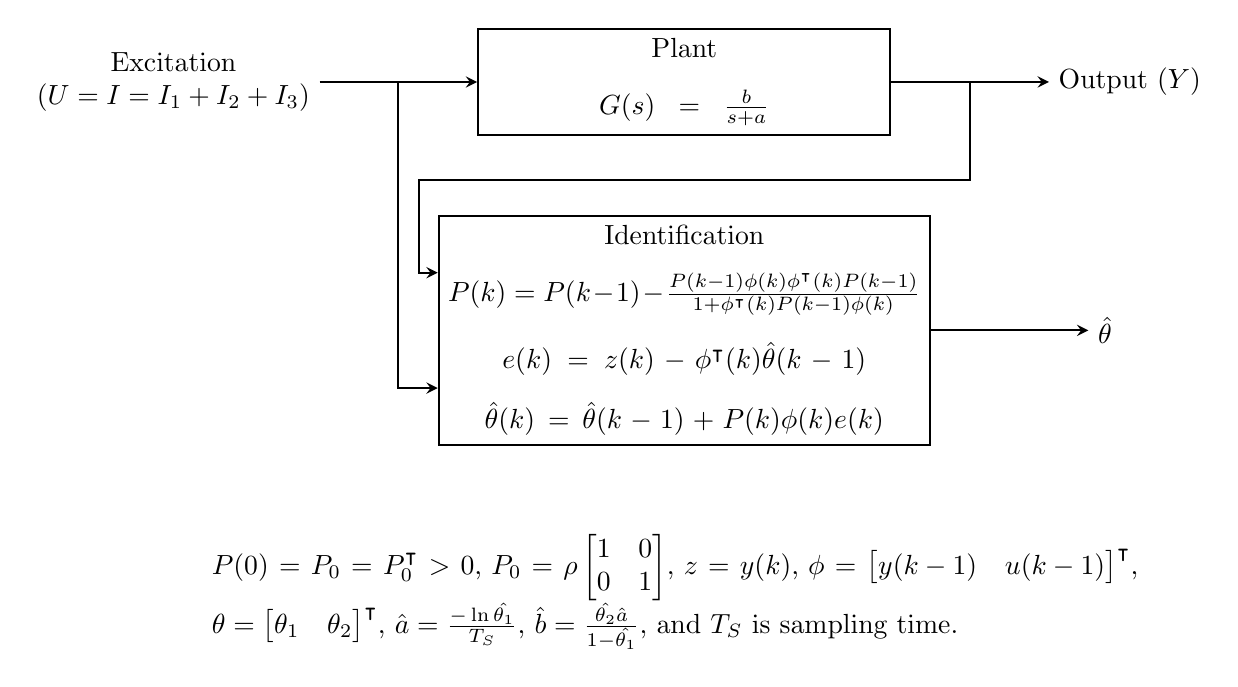
\begin{tikzpicture}[node distance = 10mm, auto]
	\node (Excitation) [align=center] {Excitation\\($U=I=I_1+I_2+I_3$)};
	\node (Plant) [block, text width = 5cm, right = of Excitation, right = 2cm] {Plant \\[0.3cm] $G(s) = \frac{b}{s+a}$};
	\node (PlantRight) [support, right = of Plant, right = 1cm] {};
	\node (PlantLeft) [support, left = of Plant, left = 1cm] {};
	\node (Identification) [block, text width = 6cm, below = of Plant] {Identification
		\\[0.3cm]
		$P(k) = P(k-1) - \frac{P(k-1)\phi(k)\phi^\intercal(k)P(k-1)}{1 + \phi^\intercal(k)P(k-1)\phi(k)}$\\[0.3cm]
		$e(k) = z(k) - \phi^\intercal(k)\hat{\theta}(k-1)$\\[0.3cm]
		$\hat{\theta}(k) = \hat{\theta}(k-1) + P(k)\phi (k)e(k)$};
	\node (Output) [right = of Plant, right = 2cm] {Output ($Y$)};
	\node (CapValues) [right = of Identification, right = 2cm] {$\hat{\theta}$};
	\path (Excitation.east) -- (Excitation.north east) coordinate[pos=0.5] (Reference1);
	\path (Identification.west) -- (Identification.north west) coordinate[pos=0.5] (Identification1);
	\path (Identification.west) -- (Identification.north west) coordinate[pos=-0.5] (Identification2);
	\draw [arrow] (Excitation) -- (Plant);
	\draw [arrow] (Plant) -- (Output);
	\draw [arrow] (PlantRight) -- +(0, -1.25) -| +(-7,-1.25) |- (Identification1);
	\draw [arrow] (PlantLeft) |- (Identification2);
	\draw [arrow] (Identification) -- (CapValues);
	\node (Equation000) [text width = 12cm, below = 1cm of Identification, align = left] {
		$P(0) = P_0 = P_0^\intercal>0$, $P_0 = \rho
		\begin{bmatrix}
			1 & 0 \\
			0 & 1
		\end{bmatrix}$,
		$z = y(k)$,
		$\phi = \begin{bmatrix}
			y(k-1) &
			u(k-1)
		\end{bmatrix}^\intercal$,
		$\theta = \begin{bmatrix}
			\theta_1 &
			\theta_2
		\end{bmatrix}^\intercal$,
		$\hat{a} = \frac{-\ln{\hat{\theta_1}}}{T_S}$,
		$\hat{b} = \frac{\hat{\theta_2}\hat{a}}{1-\hat{\theta_1}}$, and $T_S$ is sampling time.
	};
	\end{tikzpicture}
	\caption{First order system identification}
	\label{Fig:FirstOrderIdentification}
\end{figure}

\begin{figure}
	\centering
	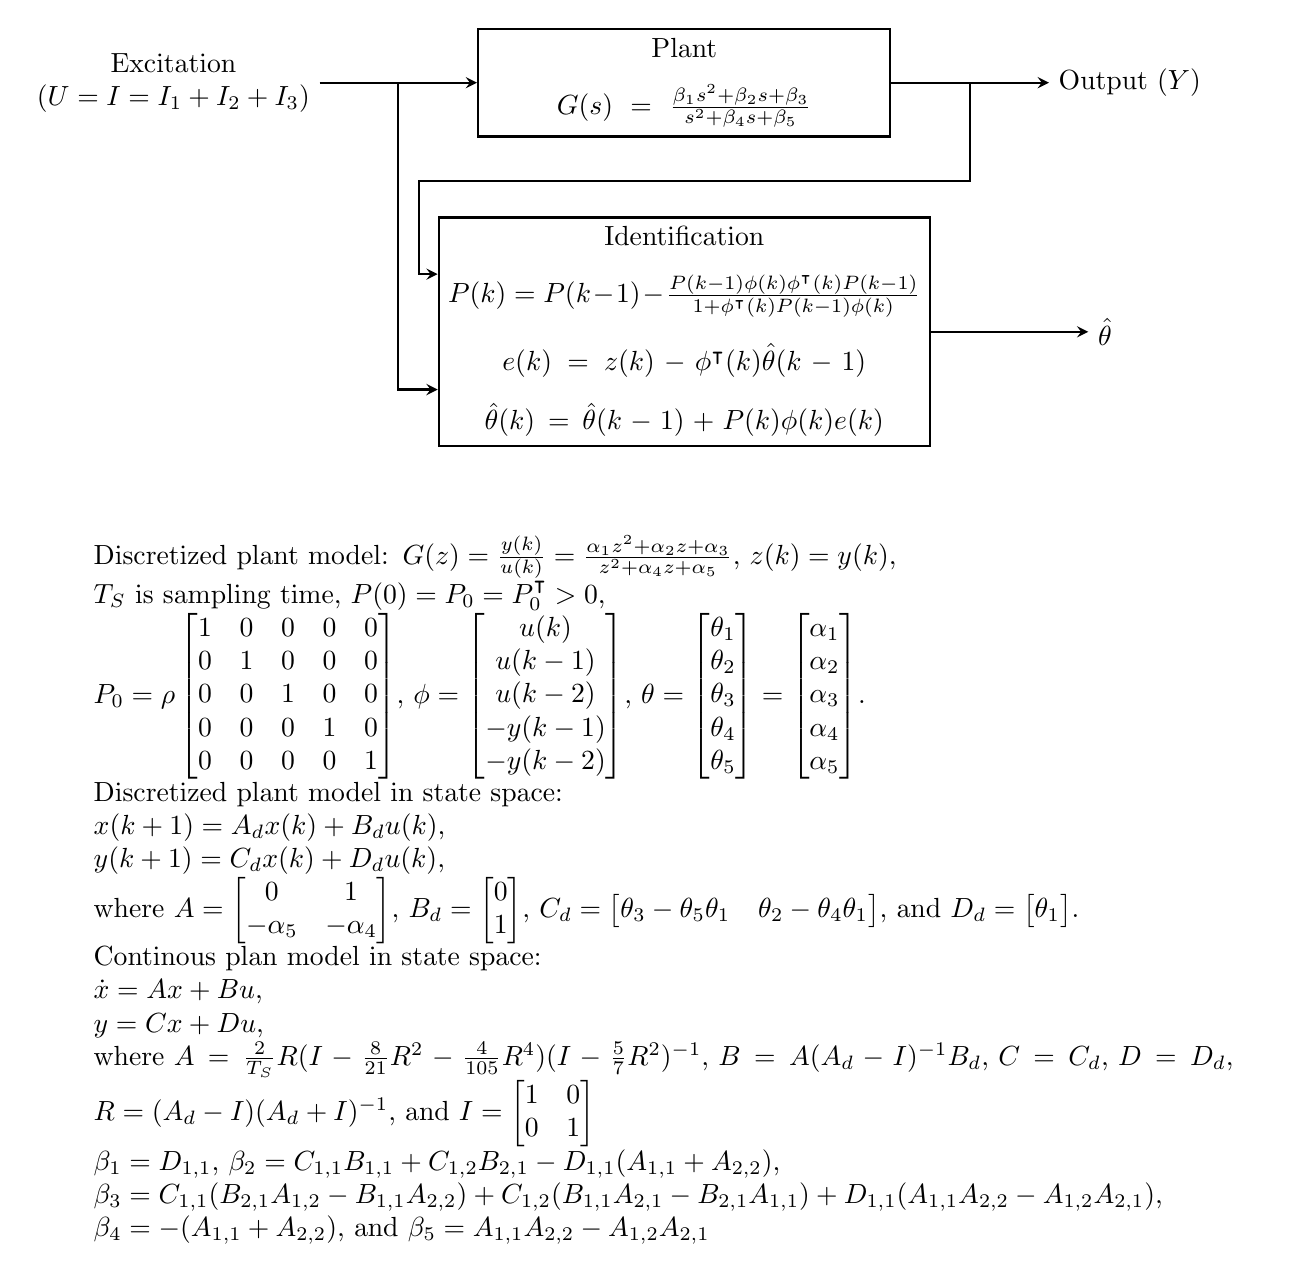
\begin{tikzpicture}[node distance = 10mm, auto]
	\node (Excitation) [align=center] {Excitation\\($U=I=I_1+I_2+I_3$)};
	\node (Plant) [block, text width = 5cm, right = of Excitation, right = 2cm] {Plant \\[0.3cm] $G(s) = \frac{\beta_1s^2 + \beta_2s + \beta_3}{s^2 + \beta_4s + \beta_5}$};
	\node (PlantRight) [support, right = of Plant, right = 1cm] {};
	\node (PlantLeft) [support, left = of Plant, left = 1cm] {};
	\node (Identification) [block, text width = 6cm, below = of Plant] {Identification
		\\[0.3cm]
		$P(k) = P(k-1) - \frac{P(k-1)\phi(k)\phi^\intercal(k)P(k-1)}{1 + \phi^\intercal(k)P(k-1)\phi(k)}$\\[0.3cm]
		$e(k) = z(k) - \phi^\intercal(k)\hat{\theta}(k-1)$\\[0.3cm]
		$\hat{\theta}(k) = \hat{\theta}(k-1) + P(k)\phi (k)e(k)$};
	\node (Output) [right = of Plant, right = 2cm] {Output ($Y$)};
	\node (CapValues) [right = of Identification, right = 2cm] {$\hat{\theta}$};
	\path (Excitation.east) -- (Excitation.north east) coordinate[pos=0.5] (Reference1);
	\path (Identification.west) -- (Identification.north west) coordinate[pos=0.5] (Identification1);
	\path (Identification.west) -- (Identification.north west) coordinate[pos=-0.5] (Identification2);
	\draw [arrow] (Excitation) -- (Plant);
	\draw [arrow] (Plant) -- (Output);
	\draw [arrow] (PlantRight) -- +(0, -1.25) -| +(-7,-1.25) |- (Identification1);
	\draw [arrow] (PlantLeft) |- (Identification2);
	\draw [arrow] (Identification) -- (CapValues);
	\node (Equation000) [text width = 15cm, below = 1cm of Identification, align = left] {
		Discretized plant model:
		$G(z)=\frac{y(k)}{u(k)} = \frac{\alpha_1z^2 + \alpha_2z + \alpha_3}{z^2 + \alpha_4z + \alpha_5}$,
		$z(k) = y(k)$,\\
		$T_S$ is sampling time, 
		$P(0) = P_0 = P_0^\intercal>0$,\\
		$P_0 = \rho
		\begin{bmatrix}
			1 & 0 & 0 & 0 & 0 \\
			0 & 1 & 0 & 0 & 0 \\
			0 & 0 & 1 & 0 & 0 \\
			0 & 0 & 0 & 1 & 0 \\
			0 & 0 & 0 & 0 & 1			
		\end{bmatrix}$,
		$\phi = \begin{bmatrix}
		u(k)\\
		u(k-1)\\
		u(k-2)\\
		-y(k-1)\\
		-y(k-2)
		\end{bmatrix}$,
		$\theta = \begin{bmatrix}
		\theta_1\\
		\theta_2\\
		\theta_3\\
		\theta_4\\
		\theta_5
		\end{bmatrix}=\begin{bmatrix}
		\alpha_1\\
		\alpha_2\\
		\alpha_3\\
		\alpha_4\\
		\alpha_5
		\end{bmatrix}$.\\
		Discretized plant model in state space:\\
		$x(k+1) = A_dx(k) + B_du(k)$,\\
		$y(k+1) = C_dx(k) + D_du(k)$,\\
		where $A=\begin{bmatrix}
			0 & 1 \\
			-\alpha_5 & -\alpha_4
		\end{bmatrix}$,
		$B_d = \begin{bmatrix}
			0\\
			1
		\end{bmatrix}$, 
		$C_d = \begin{bmatrix}
			\theta_3-\theta_5\theta_1 & \theta_2-\theta_4\theta_1
		\end{bmatrix}$, and
		$D_d = \begin{bmatrix}
			\theta_1
		\end{bmatrix}$.\\
		Continous plan model in state space:\\
		$\dot x = Ax + Bu$,\\
		$y = Cx + Du$,\\
		where $A = \frac{2}{T_S}R(I-\frac{8}{21}R^2-\frac{4}{105}R^4)(I-\frac{5}{7}R^2)^{-1}$,
		$B = A(A_d-I)^{-1}B_d$,
		$C = C_d$,
		$D = D_d$, 
		$R = (A_d-I)(A_d+I)^{-1}$, and
		$I = \begin{bmatrix}
			1 & 0\\
			0 & 1
		\end{bmatrix}$\\
		$\beta_1 = D_{1,1}$, 
		$\beta_2 = C_{1,1}B_{1,1}+C_{1,2}B_{2,1} - D_{1,1}(A_{1,1}+A_{2,2})$,\\
		$\beta_3 = C_{1,1}(B_{2,1}A_{1,2}- B_{1,1}A_{2,2}) + C_{1,2}(B_{1,1}A_{2,1}-B_{2,1}A_{1,1}) + D_{1,1}(A_{1,1}A_{2,2}-A_{1,2}A_{2,1})$,\\
		$\beta_4 = -(A_{1,1}+A_{2,2})$, and
		$\beta_5 = A_{1,1}A_{2,2} - A_{1,2}A_{2,1}$
	};
	\end{tikzpicture}
	\caption{Second order system identification}
	\label{Fig:SecondOrderIdentification}
\end{figure}

\begin{figure}
	\centering
	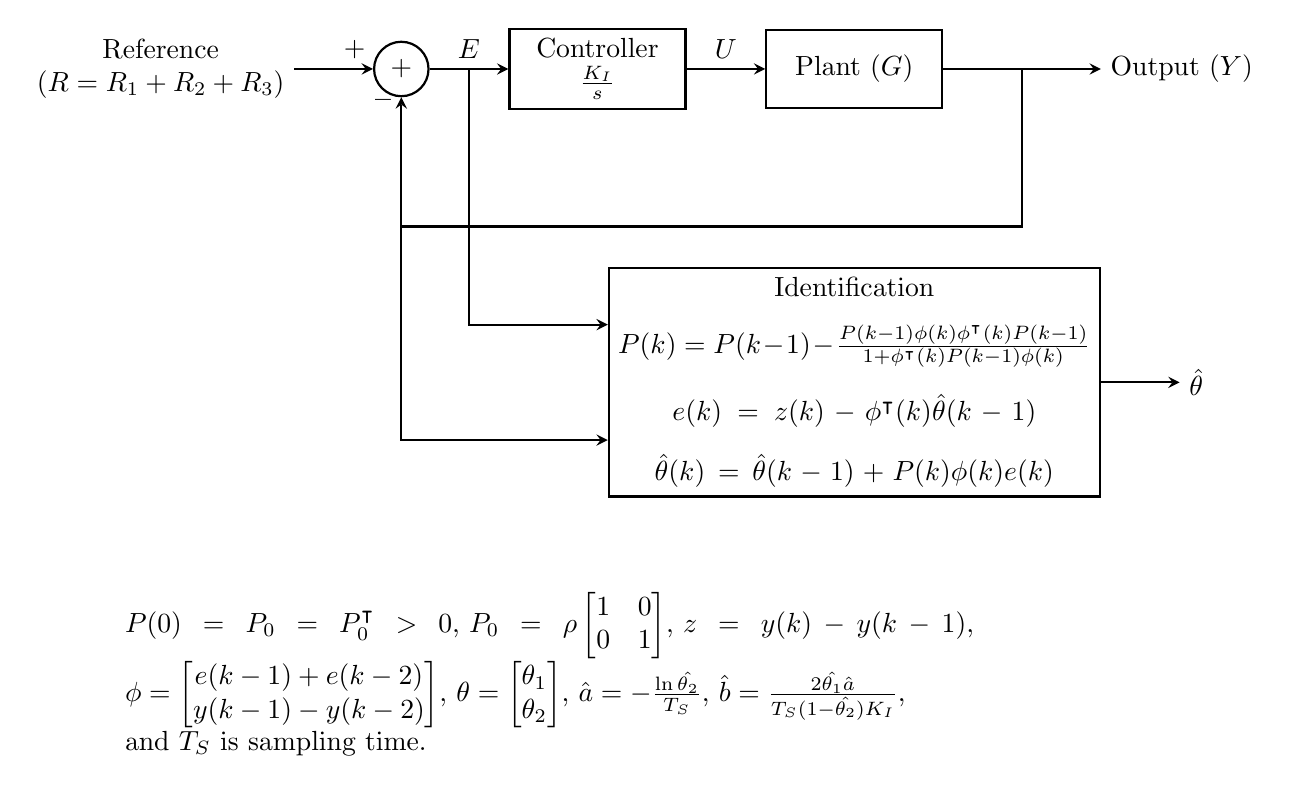
\begin{tikzpicture}[node distance = 10mm, auto]
	\node (Reference) [align=center] {Reference\\($R=R_1+R_2+R_3$)};
	\node (SummingPoint) [draw,circle, thick, right = of Reference]  {+};
	\node (Control) [block, text width = 2cm, right = of SummingPoint] {Controller\\$\frac{K_I}{s}$};
	\node (ControlLeft) [support, left = of Control, left = 0.5cm] {};
	\node (Plant) [block, text width = 2cm, right = of Control] {Plant ($G$)};
	\node (PlantRight) [support, right = of Plant, right = 1cm] {};
	\node (Output) [right = of Plant, right = 2cm] {Output ($Y$)};
	\node (Identification) [block, text width = 6cm, below = 2cm of Plant] {Identification
	\\[0.3cm]
	$P(k) = P(k-1) - \frac{P(k-1)\phi(k)\phi^\intercal(k)P(k-1)}{1 + \phi^\intercal(k)P(k-1)\phi(k)}$\\[0.3cm]
	$e(k) = z(k) - \phi^\intercal(k)\hat{\theta}(k-1)$\\[0.3cm]
	$\hat{\theta}(k) = \hat{\theta}(k-1) + P(k)\phi (k)e(k)$};
	\node (OutputTapingPoint) [support, below = of SummingPoint] {};
	\node (CapValues) [right = of Identification, right = 1cm] {$\hat{\theta}$};
	\draw [arrow] (Reference) -- node[anchor=south west]{+}(SummingPoint);
	\draw [arrow] (SummingPoint) -- node[anchor=south]{$E$}(Control);
	\draw [arrow] (Control) -- node[anchor=south]{$U$}(Plant);
	\draw [arrow] (Plant) -- (Output);
	\draw [arrow] (PlantRight) -- +(0, -2) -| (SummingPoint) node[below = 2mm, anchor=north east]{\bf\textendash};
	\path (Identification.west) -- (Identification.north west) coordinate[pos=0.5] (Identification1);
	\path (Identification.west) -- (Identification.north west) coordinate[pos=-0.5] (Identification2);
	\draw [arrow] (ControlLeft) |- (Identification1);
	\draw [arrow] (OutputTapingPoint) |- (Identification2);
	\draw [arrow] (Identification) -- (CapValues);
	\node (Equation000) [text width = 12cm, below = 6cm of Control, align = left] {
		$P(0) = P_0 = P_0^\intercal>0$, $P_0 = \rho
		\begin{bmatrix}
		1 & 0 \\
		0 & 1
		\end{bmatrix}$,
		$z = y(k) - y(k-1)$,
		$\phi = \begin{bmatrix}
		e(k-1) + e(k-2) \\
		y(k-1) - y(k-2)
		\end{bmatrix}$,
		$\theta = \begin{bmatrix}
		\theta_1 \\
		\theta_2
		\end{bmatrix}$,
		$\hat{a} = -\frac{\ln{\hat{\theta_2}}}{T_S}$,
		$\hat{b} = \frac{2\hat{\theta_1}\hat{a}}{T_S(1-\hat{\theta_2})K_I}$,\\
		and $T_S$ is sampling time.
	};
	\end{tikzpicture}
	\caption{Parameter estimation of a first order system with integral controller}
	\label{Fig:IdentificationWithIntegralController}
\end{figure}

%\bibliographystyle{apacite}%unsrtnat}
%\bibliographystyle{spbasic}      % basic style, author-year citations
%\bibliographystyle{spmpsci}      % mathematics and physical sciences
%\bibliographystyle{spphys}       % APS-like style for physics
%\bibliographystyle{ieeetr}
%\bibliography{refs}
\end{document}